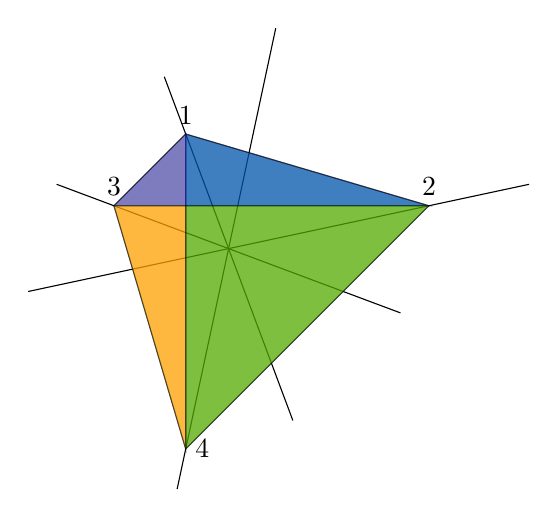
\begin{tikzpicture}[scale=2]

\coordinate [label=above:2] (1) at (1, 0, {-1 / sqrt(2)});
\coordinate [label=above:3] (2) at (-1, 0, -{1 / sqrt(2)});
\coordinate [label=above:1] (3) at (0, 1, {1 / sqrt(2)});
\coordinate [label=right:4] (4) at (0, -1, {1 / sqrt(2)});

\draw[-] (1.5, 0, {-1.5 / sqrt(2)})--(-1, 0, {1 / sqrt(2)});
\draw[-] (-1.5, 0, -{1.5 / sqrt(2)})--(1.5, 0, {1.5 / sqrt(2)});
\draw[-] (0, 1.5, {1.5 / sqrt(2)})--(0, -1.5, {-1.5 / sqrt(2)});
\draw[-] (0, -1.2, {1.2 / sqrt(2)})--(0, 1.1, {-1.1 / sqrt(2)});

\draw[-, fill=red, opacity=.5] (1)--(4)--(2)--cycle;
\draw[-, fill=green, opacity=.5] (1)--(4)--(3)--cycle;
\draw[-, fill=yellow, opacity=.5] (2)--(4)--(3)--cycle;
\draw[-, fill=blue, opacity=.5] (1)--(2)--(3)--cycle;


\end{tikzpicture}